\chapter{Analiza tematu}
\label{ch:analiza}

\section{Miejsce kodowania kanałowego w~torze PDSCH}
\label{sec:analiza_kontekst}

W 5G NR dane użytkownika w~łączu w~dół są przenoszone w~kanale transportowym DL-SCH (Downlink Shared Channel), a~następnie transmitowane w~kanale fizycznym PDSCH. Z punktu widzenia toru nadajnika oznacza to, że zanim informacja zostanie zamieniona na symbole modulacji i~umieszczona w~zasobach czasowo--częstotliwościowych, przechodzi przez sekwencję kroków przetwarzania warstwy fizycznej. Kluczowym elementem tego łańcucha jest kodowanie kanałowe, którego zadaniem jest zwiększenie odporności transmisji na błędy w~kanale radiowym \cite{bib:3gpp_38212}.

Całościowo proces przygotowania danych do transmisji w~PDSCH można opisać następującymi etapami (zgodnie z~kolejnością wykonywania):
\begin{enumerate}
  \item \textbf{Dołączenie CRC do TB (\english{Transport Block} - blok transportowy)} -- wyznaczenie sumy kontrolnej i~dopisanie jej do danych TB.
  \item \textbf{Wybór parametrów kodowania LDPC} determinujących strukturę kodu.
  \item \textbf{Segmentacja TB na CB (\english{Code Block/Blocks} - blok kodowy/bloki kodowe)} oraz (w razie potrzeby) \textbf{dołączenie CRC dla CB}, aby umożliwić kodowanie LDPC w~ograniczonych długościach wejściowych.
  \item \textbf{Kodowanie kanałowe LDPC} każdego CB, prowadzące do powstania bitów parzystości i~słowa kodowego.
  \item \textbf{Rate matching} -- dopasowanie liczby bitów po kodowaniu do dostępnych zasobów transmisyjnych.
  \item \textbf{Konkatenacja} -- połączenie przetworzonych bloków kodowych w~jeden strumień bitów na wyjściu części kodującej.
  \item \textbf{\english{Scrambling}} -- losowanie (pseudolosowe) strumienia bitów w~celu ograniczenia niekorzystnych własności sekwencji i~poprawy właściwości transmisyjnych.
  \item \textbf{Modulacja} -- mapowanie bitów na symbole modulacji (np. QPSK/16QAM/64QAM/256QAM).
  \item \textbf{Mapowanie warstw} oraz \textbf{mapowanie na porty antenowe} -- rozdział symboli na warstwy i~porty.
  \item \textbf{Mapowanie na zasoby radiowe} -- rozmieszczenie symboli w~elementach zasobów, w~tym przypisanie do bloków zasobów i~dalsze przetwarzanie prowadzące do sygnału OFDM.
\end{enumerate}

W niniejszej pracy analizowany i~implementowany jest fragment, toru odpowiadający za kodowanie kanałowe dla PDSCH, tj. etapy obejmujące dołączenie CRC, segmentację na CB, kodowanie LDPC oraz przygotowanie strumienia w~zakresie wymaganym do uzyskania poprawnych danych wyjściowych \cite{bib:3gpp_38212}. Etapy związane z~mieszaniem, modulacją, mapowaniem na warstwy/porty oraz mapowaniem na zasoby i~generacją sygnału OFDM, pozostają poza zakresem projektu i~są traktowane jako kolejne kroki realizowane po stronie nadajnika \cite{bib:3gpp_38211}.

Spotyka się również opracowania poglądowe, przedstawiające cały łańcuch przetwarzania PDSCH wraz ze wskazaniem odpowiadających mu rozdziałów specyfikacji 3GPP\cite{bib:sharetechnote_pdsch}. Tego typu materiały mogą służyć jako wizualne uzupełnienie opisu oraz ułatwienie interpretacji standardu, jednak podstawą definicji algorytmów w~niniejszej pracy są dokumenty normatywne 3GPP \cite{bib:3gpp_38212,bib:3gpp_38211}.


\section{Blok transportowy i~sumy kontrolne CRC}
\label{sec:analiza_crc}

W 5G NR podstawową jednostką danych przekazywaną do toru kodowania kanałowego dla PDSCH jest TB. TB stanowi ciąg bitów pochodzących z~warstwy wyższej, który w~nadajniku podlega operacjom zwiększającym niezawodność transmisji, a~następnie jest przygotowywany do mapowania na kanał fizyczny. Jednym z~pierwszych kroków po stronie nadajnika jest dołączenie sumy kontrolnej CRC, której celem jest wykrywanie błędów po~stronie odbiornika (CRC nie służy do korekcji błędów, a~jedynie do ich detekcji) \cite{bib:3gpp_38212}.

Proces dołączenia CRC do TB polega na wyznaczeniu reszty z~dzielenia wielomianowego (modulo-2) danych przez wielomian generatora CRC, a~następnie dopisaniu uzyskanych bitów na końcu bloku. Specyfikacja 3GPP definiuje stosowane warianty CRC oraz odpowiadające im wielomiany generatora \cite{bib:3gpp_38212}. W dalszej części pracy przyjmuje się następujące oznaczenia długości:
\begin{itemize}
  \item $A$ -- liczba bitów TB przed dołączeniem CRC,
  \item $L$ -- długość CRC dołączanego do TB,
  \item $B$ -- liczba bitów po dołączeniu CRC.
\end{itemize}
Zależność pomiędzy tymi wielkościami ma postać:
\begin{equation}
B = A + L.
\label{eq:tb_crc_length}
\end{equation}

Długość CRC dołączanego do TB zależy od długości $A$ i~jest określona w~specyfikacji 3GPP TS~38.212. W typowym przypadku stosuje się CRC16 dla krótszych bloków transportowych oraz CRC24A dla dłuższych TB, zgodnie z~progiem długości TB zdefiniowanym w~standardzie \cite{bib:3gpp_38212}. Dołączenie CRC na poziomie TB umożliwia weryfikację poprawności całego bloku transportowego po stronie odbiornika.

W kolejnych etapach toru kodowania TB może zostać podzielony na CB. Jeżeli segmentacja jest wymagana, standard przewiduje również dołączenie dodatkowej sumy kontrolnej CRC na poziomie każdego CB, co pozwala na niezależną detekcję błędów w~poszczególnych blokach kodowych \cite{bib:3gpp_38212}.


\section{Dobór parametrów kodowania LDPC}
\label{sec:analiza_parametry_ldpc}

Kodowanie kanałowe realizowane jest z~wykorzystaniem kodów LDPC o~strukturze quasi-cyklicznej (QC-LDPC). W praktyce oznacza to, że właściwe kodowanie odbywa się na poziomie bloków kodowych, jednak już przed segmentacją należy wyznaczyć parametry, które determinują dopuszczalne długości wejściowe CB oraz strukturę macierzy parzystości, a~tym samym wpływają na samą segmentację \cite{bib:3gpp_38212}.

\subsection{Założenia wejściowe i~pojęcie docelowego współczynnika kodowania}
Dobór parametrów LDPC jest powiązany z~konfiguracją transmisji, która determinuje docelową liczbę bitów przeznaczonych do transmisji oraz efektywny współczynnik kodowania. Zasady doboru parametrów transmisji opisuje 3GPP TS~38.214 \cite{bib:3gpp_38214}. W dalszych rozważaniach przyjmuje się, że na wejściu procedury doboru parametrów znana jest:
\begin{itemize}
  \item długość bloku transportowego: $A$,
  \item docelowy (efektywny) współczynnik kodowania, oznaczony jako $R$.
\end{itemize}

Kolejność kroków oraz zależności pomiędzy parametrami przedstawiono na rys.~\ref{fig:flowchart_ldpc_params}.


% --- Flowchart: procedura doboru parametrów (wstawka w~środku sekcji) ---
\begin{figure}
  \centering
  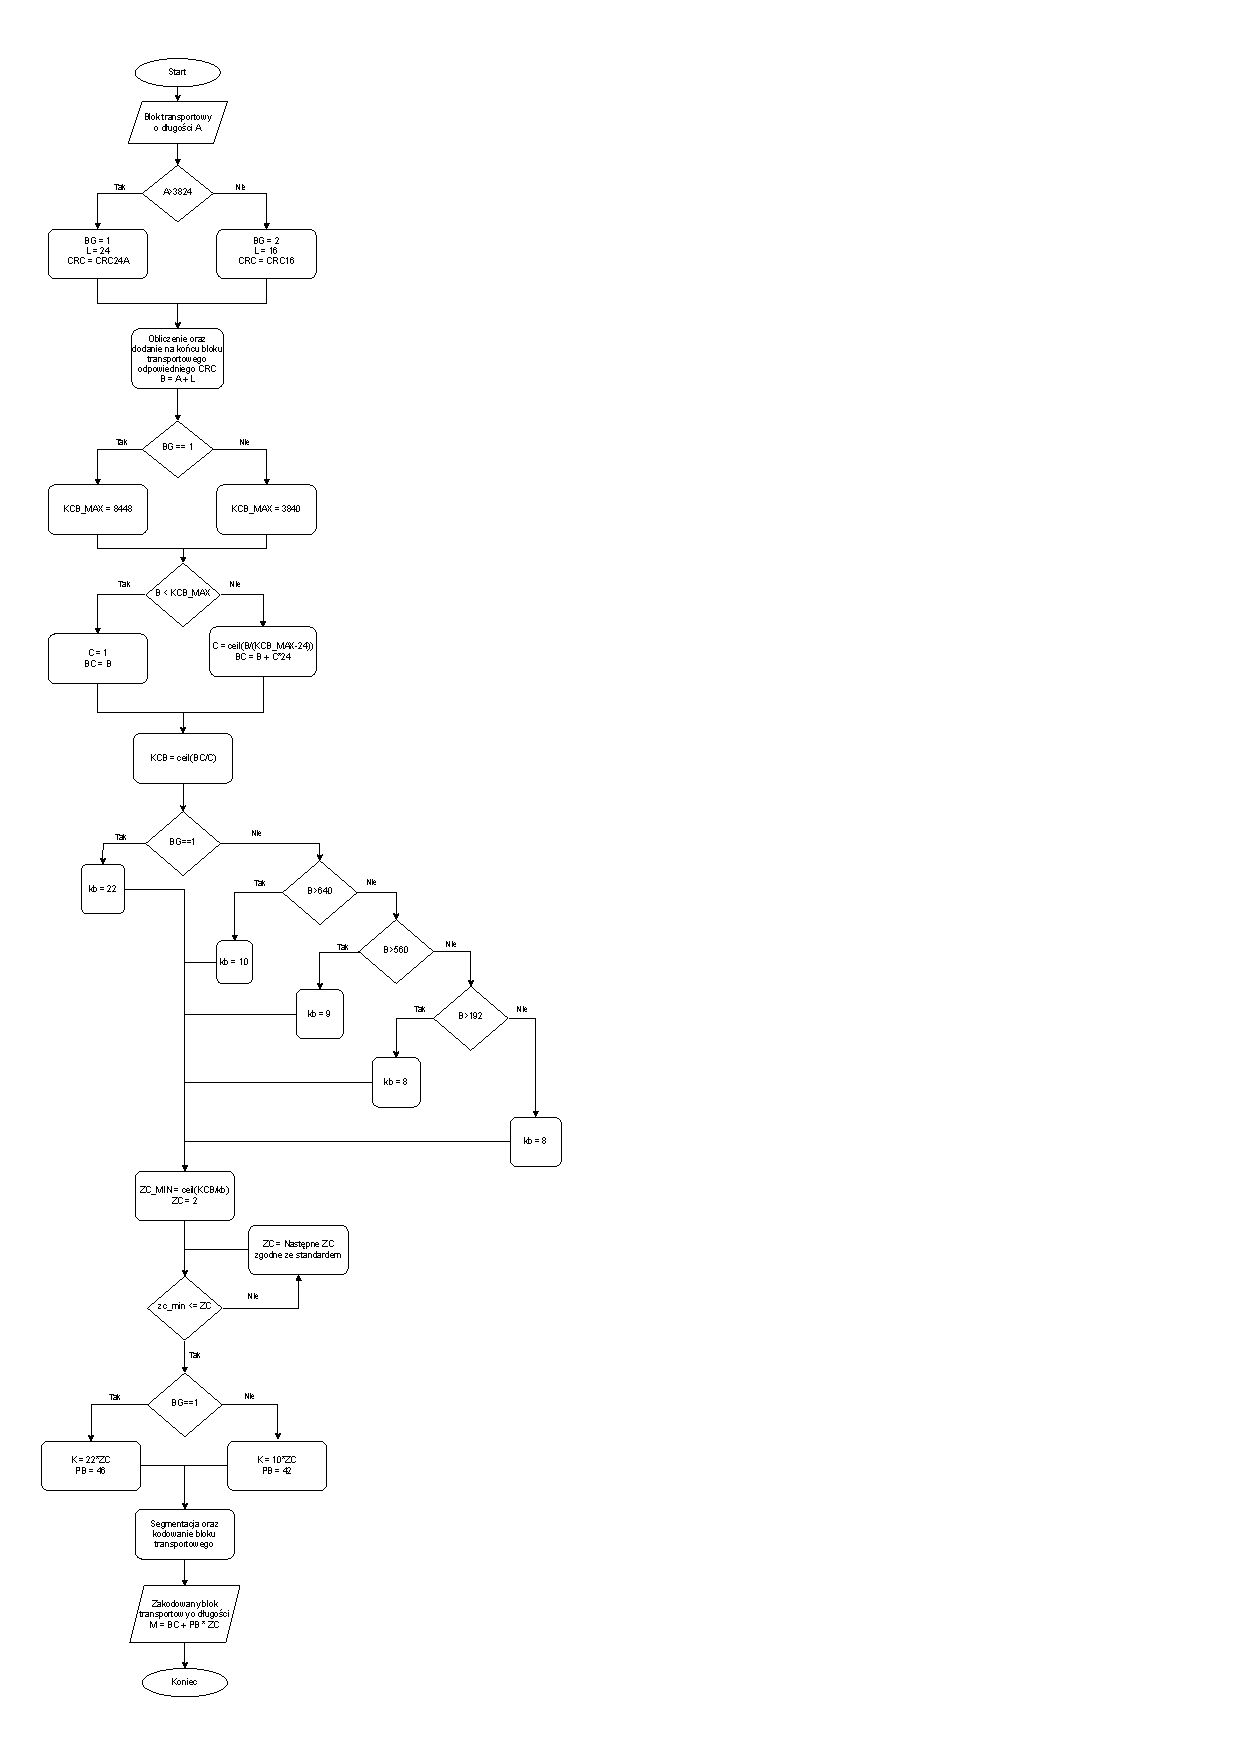
\includegraphics[width=0.95\textwidth]{schematy/Flowchart.pdf}
  \caption{Procedura doboru parametrów segmentacji oraz kodowania LDPC.}
  \label{fig:flowchart_ldpc_params}
\end{figure}

\subsection{Wybór grafu bazowego}
Standard 3GPP definiuje dwa grafy bazowe kodu LDPC: BG1 oraz BG2. Wybór grafu bazowego wpływa na:
\begin{itemize}
  \item dopuszczalne zakresy długości wejściowych bloków kodowych,
  \item strukturę (rozmiar) macierzy bazowej, a~w~konsekwencji liczbę bloków parzystości,
  \item listę oraz sposób doboru parametrów pośrednich, używanych przy wyborze rzędu \english{liftingu}.
\end{itemize}
Reguły wyboru grafu bazowego w~standardzie 3GPP są powiązane z~długością danych oraz docelowym współczynnikiem kodowania, a~szczegółowe warunki wyboru podano w~TS~38.212. W niniejszej pracy, ze względu na przyjęty zakres implementacji i~brak pełnego mechanizmu \english{rate matching'u}, zastosowano uproszczenie polegające na uzależnieniu wyboru BG wyłącznie od długości bloku transportowego przed dołączeniem CRC, tj. parametru $A$. \cite{bib:3gpp_38212}.

\subsection{Lifting i~dobór wartości $Z_c$}
Po wyborze grafu bazowego konieczne jest wyznaczenie wartości $Z_c$, która opisuje rozmiar podmacierzy w~strukturze QC-LDPC. Lifting jest procesem rozszerzania strukturalnego macierzy bazowej kodu LDPC poprzez jej zastąpienie blokową macierzą permutacji, w~których poszczególne bloki są kwadratowymi podmacierzami o~rozmiarze $Z_c \times Z_c$. Wartość $Z_c$ jest wybierana z~dyskretnej listy wartości dopuszczonych w~standardzie \cite{bib:3gpp_38212}.

Parametr $k_b$ jest wielkością zdefiniowaną w~TS~38.212 i~pełni rolę parametru pośredniego w~procedurze doboru wartości $Z_c$. Mówi on ile spośród $K_b$ bloków części informacyjnej posiada dane TB. Pozostałe bloki zawierają tylko wypełnienie. Wartość $K_b$ jest stała i~wynosi 22 dla BG1 oraz 10 dla BG2. W strukturze QC-LDPC wejściowy wektor informacji dla pojedynczego bloku kodowego ma długość:
\begin{equation}
K = K_b \cdot Z_c,
\label{eq:K_kbZc}
\end{equation}

Powyższe można interpretować jako $K_b$ bloków kolumnowych po $Z_c$ bitów każdy, tworzących część informacyjną słowa kodowego. W praktyce oznacza to, że po segmentacji do kodera dla danego CB wprowadzana jest sekwencja o~docelowej długości $K_{\mathrm{CB}}$ bitów, która zajmuje tylko część z~dostępnych $K_b \cdot Z_c$ pozycji. Pozostałe pozycje na potrzeby obliczeń są wypełniane bitami wypełniającymi (\emph{filler bits}), które służą wyłącznie do wyrównania długości do wymaganej struktury QC i~nie są transmitowane. Następnie:
\begin{equation}
  Z_{c\_min} = \left\lceil \frac{K_{\mathrm{CB}}}{k_b} \right\rceil,
  \label{eq:zc_min}
\end{equation}
gdzie $K_{\mathrm{CB}}$ oznacza docelową długość informacji dla pojedynczego CB (wyznaczaną na etapie segmentacji), a~$k_b$ jest parametrem określonym w~TS~38.212 \cite{bib:3gpp_38212}. Ostatecznie wybiera się $Z_c$ jako najmniejszą wartość z~listy dopuszczalnych, spełniającą warunek:
\begin{equation}
  Z_c \ge Z_{c\_min}.
  \label{eq:zc_choice}
\end{equation}

\subsection{Zależność doboru parametrów LDPC od segmentacji}
Dobór grafu bazowego i~$Z_c$ determinuje ograniczenia dotyczące długości wejściowej CB (w szczególności $K_{\mathrm{CB\_max}}$ zależne od BG) oraz strukturę słowa kodowego po kodowaniu LDPC. W konsekwencji, znając $B$ oraz zasady doboru BG i~$Z_c$, można w~kolejnym kroku wyznaczyć liczbę bloków kodowych $C$ oraz długości bloków po segmentacji w~sposób zgodny ze specyfikacją.\cite{bib:3gpp_38212}.





\section{Segmentacja}
\label{sec:analiza_segmentacja}

Po dołączeniu CRC do bloku transportowego otrzymuje się sekwencję długości $B$ bitów, stanowiącą wejście do procedury segmentacji na bloki kodowe. Segmentacja jest wymagana, ponieważ koder LDPC pracuje na blokach o~ograniczonej długości wejściowej, zależnej od wybranego grafu bazowego \cite{bib:3gpp_38212}.

\subsection{Maksymalna długość bloku kodowego}
Standard definiuje maksymalny rozmiar wejściowy bloku kodowego $K_{\mathrm{CB\_max}}$ zależny od grafu bazowego:
\begin{itemize}
  \item dla BG1: $K_{\mathrm{CB\_max}} = 8448$,
  \item dla BG2: $K_{\mathrm{CB\_max}} = 3840$.
\end{itemize}
Wartości te determinują, czy segmentacja jest wykonywana oraz ile bloków kodowych należy utworzyć \cite{bib:3gpp_38212}.

\subsection{Wyznaczenie liczby bloków kodowych i~narzutu CRC dla CB}
Jeżeli $B \le K_{\mathrm{CB\_max}}$, segmentacja nie jest wymagana i~przyjmuje się:
\begin{equation}
C = 1,\qquad L_{\mathrm{CB}} = 0,\qquad B' = B,
\label{eq:seg_case_no}
\end{equation}
gdzie $C$ oznacza liczbę bloków kodowych, $L_{\mathrm{CB}}$ długość CRC dołączanego do każdego CB, a~$B'$ długość sekwencji po uwzględnieniu ewentualnych CRC na poziomie CB \cite{bib:3gpp_38212}.

W przeciwnym razie standard przewiduje segmentację i~dołączenie CRC o~długości $L_{\mathrm{CB}} = 24$ bitów do każdego CB. Wówczas:
\begin{equation}
C = \left\lceil \frac{B}{K_{\mathrm{CB\_max}} - L_{\mathrm{CB}}} \right\rceil,\qquad
B' = B + C \cdot L_{\mathrm{CB}}.
\label{eq:seg_case_yes}
\end{equation}
W 5G NR dla CB-CRC stosowany jest wielomian generatora CRC24B, zgodnie z~TS~38.212 \cite{bib:3gpp_38212}.

\subsection{Podział bitów na CB oraz bity wypełniające (\english{filler bits})}
Po wyznaczeniu $C$ i~$B'$ określa się nominalną długość danych przypadającą na jeden blok kodowy:
\begin{equation}
K_{\mathrm{CB}} = \left\lceil\frac{B'}{C}\right\rceil.
\label{eq:seg_kprime}
\end{equation}
Następnie bity wejściowe są rozdzielane kolejno do bloków $c_r$, gdzie $r \in \{0,\dots,C-1\}$, a~gdy $C>1$ do każdego bloku dopisywane są bity CRC24B \cite{bib:3gpp_38212}.

W kolejnym kroku, aby dopasować długość wejściową kodera QC-LDPC do struktury wynikającej z~\english{lifting'u}, do każdego bloku mogą zostać dopisane bity wypełniające. Są to bity nieprzeznaczone do transmisji, a~tylko na potrzeby kodowania w~ich miejsce wstawiane są binarne wartości równe 0. Ich rolą jest wyrównanie długości bloku do wymaganej wartości:
\begin{equation}
K = K_b \cdot Z_c,\qquad K \ge K_{\mathrm{CB}},
\label{eq:seg_k_lift}
\end{equation}
gdzie $K_b$ i~$Z_c$ są zdefiniowane w~TS~38.212, a~liczba bitów wypełniających jest równa $F = K - K_{\mathrm{CB}}$ \cite{bib:3gpp_38212}.

Wynikiem segmentacji jest zatem zbiór $C$ bloków kodowych o~długości $K$ (po uwzględnieniu CRC na poziomie CB i~ewentualnych \english{filler bits}), które stanowią bezpośrednie wejście do etapu kodowania LDPC.




\section{Proces kodowania LDPC}
\label{sec:analiza_proces_kodowania_ldpc}

Kodowanie LDPC w~5G NR dla DL-SCH/PDSCH realizowane jest w~postaci kodów quasi-cyklicznych (QC-LDPC),
w których macierz kontroli parzystości \textbf{H} jest zbudowana z~podmacierzy będących macierzami permutacji cyklicznych o~rozmiarze $Z_c \times Z_c$ lub macierzami zerowymi. Własność quasi-cykliczna sprawia,
że mnożenie przez podmacierze nie wymaga klasycznych operacji macierzowych, a~sprowadza się do operacji przesunięć cyklicznych
i sumowania modulo-2 (XOR) na wektorach o~długości $Z_c$.

\subsection{Warunek parzystości i~postać słowa kodowego}
Słowo kodowe LDPC musi spełniać równanie kontroli parzystości:
\begin{equation}
\mathbf{H} \cdot \mathbf{c}^\mathbf{T} = \mathbf{0}^\mathbf{T},
\label{eq:ldpc_parity_check}
\end{equation}
gdzie $\mathbf{c}$ jest wektorem słowa kodowego, a~działania wykonywane są w~ciele $\mathrm{GF}(2)$ (czyli operacja sumy logicznej jest zastąpiona przez XOR).
W kodowaniu systematycznym słowo kodowe przyjmuje postać:
\begin{equation}
\mathbf{c} = \left[\mathbf{s} \ \mathbf{p}\right],
\label{eq:codeword_systematic}
\end{equation}
gdzie $\mathbf{s}$ zawiera bity informacyjne (po segmentacji oraz po uwzględnieniu \english{filler bits}), natomiast $\mathbf{p}$ to bity parzystości.

Ze względu na strukturę 5G NR QC-LDPC wygodnie jest grupować bity w~bloki o~długości $Z_c$:
\begin{equation}
\mathbf{s} = \left[\mathbf{s}_1,\mathbf{s}_2,\ldots,\mathbf{s}_{K_b}\right],
\label{eq:s_blocks}
\end{equation}
gdzie $K_b$ jest liczbą kolumn informacyjnych dla wybranego grafu bazowego, a~każdy
$\mathbf{s}_i$ ma długość $Z_c$. Analogicznie, parzystości można traktować jako bloki $\mathbf{p}_j$ o~długości $Z_c$.

\subsection{Podział macierzy \textbf{H} i~idea wyznaczania parzystości}
Dla 5G NR QC-LDPC macierz \textbf{H} można (na potrzeby opisu kodowania) traktować jako złożoną z~części odpowiadającej bitom
systematycznym oraz części odpowiadającej parzystości. W literaturze opisującej wydajne kodery 5G NR często wykorzystuje się
podział na dwie grupy parzystości: pierwsze $g=4$ bloków parzystości (oznaczane dalej jako $\mathbf{p}_a$) oraz pozostałe bloki
parzystości (oznaczane jako $\mathbf{p}_c$) \cite{bib:nguyen2019_qcldpc}.
Wektor słowa kodowego można wtedy zapisać jako:
\begin{equation}
\mathbf{c} = \left[\mathbf{s} \ \mathbf{p}_a \ \mathbf{p}_c\right],
\label{eq:codeword_split}
\end{equation}
a równanie \eqref{eq:ldpc_parity_check} rozdzielić na dwa kroki:
\begin{itemize}
  \item najpierw wyznaczenie czterech pierwszych bloków parzystości $\mathbf{p}_a$,
  \item następnie wyznaczenie pozostałych bloków $\mathbf{p}_c$ na podstawie $\mathbf{s}$ oraz $\mathbf{p}_a$.
\end{itemize}
Takie podejście jest zgodne z~typową implementacją sprzętową dla 5G NR, ponieważ pozwala obliczać parzystości
przy użyciu przesunięć cyklicznych oraz akumulatorów XOR, bez konstruowania macierzy generatora \cite{bib:nguyen2019_qcldpc}.

\subsection{Operacje elementarne: przesunięcie cykliczne i~akumulacja XOR}
Każdy niezerowy element macierzy bazowej odpowiada podmacierzy, będącej przesuniętą cyklicznie macierzą jednostkową
o rozmiarze $Z_c \times Z_c$. W praktyce oznacza to, że dla bloku $\mathbf{x}$ długości $Z_c$ oraz wartości przesunięcia $\rho$
wynik mnożenia przez podmacierz jest równoważny przesunięciu cyklicznemu:
\begin{equation}
\mathbf{y} = \mathrm{rot}(\mathbf{x},\rho),
\label{eq:rot}
\end{equation}
a suma wielu składników jest realizowana jako XOR wektorów:
\begin{equation}
\mathbf{u} = \bigoplus_{m} \mathbf{y}_m.
\label{eq:xor_sum}
\end{equation}

Zatem obliczanie parzystości sprowadza się do: (1) pobrania odpowiednich bloków $\mathbf{s}_i$ lub wcześniej wyznaczonych
bloków parzystości, (2) wykonania na nich przesunięć $\mathrm{rot}(\cdot)$ zgodnie z~wartościami z~macierzy bazowej,
oraz (3) zsumowania wyników operacją XOR.

\subsection{Wyznaczanie pierwszych bloków parzystości}
Pierwszy etap kodowania polega na obliczeniu czterech bloków parzystości $\mathbf{p}_a = [\mathbf{p}_{a1},\mathbf{p}_{a2},\mathbf{p}_{a3},\mathbf{p}_{a4}]$.
Dla każdego z~$g=4$ równań parzystości definiuje się akumulacje (wektory pośrednie) powstałe z~przesuniętych bloków informacji:
\begin{equation}
\boldsymbol{\lambda}_i = \bigoplus_{j=1}^{k_b} \mathrm{rot}\!\left(\mathbf{s}_j, \rho_{i,j}\right), \quad i~\in \{1,2,3,4\},
\label{eq:lambda_def}
\end{equation}
gdzie $\rho_{i,j}$ oznacza przesunięcie wynikające z~odpowiedniej pozycji w~macierzy bazowej (dla danego grafu bazowego i~$Z_c$).
Następnie $\mathbf{p}_{a1}$ jest wyznaczane jako XOR wszystkich $\boldsymbol{\lambda}_i$, a~pozostałe $\mathbf{p}_{a2}$--$\mathbf{p}_{a4}$
otrzymuje się z~prostych zależności liniowych (XOR i~ewentualne przesunięcie cykliczne wybranych bloków), wynikających z~tego,
że część odpowiadająca pierwszym parzystościom ma w~5G NR strukturę sprzyjającą wydajnej implementacji \cite{bib:nguyen2019_qcldpc}.

\subsection{Wyznaczanie pozostałych bloków parzystości}
Drugi etap kodowania wyznacza bloki $\mathbf{p}_c$ na podstawie informacji $\mathbf{s}$ oraz wcześniej obliczonych bloków $\mathbf{p}_a$.
Każdy kolejny blok parzystości jest sumą (XOR) przesuniętych cyklicznie bloków informacji oraz przesuniętych bloków $\mathbf{p}_a$:
\begin{equation}
\mathbf{p}_{c,t} =
\left(\bigoplus_{j=1}^{k_b} \mathrm{rot}\!\left(\mathbf{s}_j, \alpha_{t,j}\right)\right)
\oplus
\left(\bigoplus_{j=1}^{g} \mathrm{rot}\!\left(\mathbf{p}_{a j}, \beta_{t,j}\right)\right),
\label{eq:pc_def}
\end{equation}
gdzie $\alpha_{t,j}$ i~$\beta_{t,j}$ są przesunięciami wynikającymi z~macierzy bazowej. W praktyce oznacza to, że po obliczeniu $\mathbf{p}_a$
pozostałe parzystości można generować sekwencyjnie (blok po bloku), wykorzystując tę samą operację elementarną:
\emph{rotacja + akumulacja XOR} \cite{bib:nguyen2019_qcldpc}.



Podsumowując, kodowanie LDPC w~5G NR można interpretować jako rozwiązywanie układu równań parzystości \eqref{eq:ldpc_parity_check},
gdzie dzięki strukturze QC-LDPC operacje są realizowane przy użyciu przesunięć cyklicznych i~XOR. Umożliwia to implementację
wydajnego kodera bez przechowywania gęstej macierzy generatora, co jest szczególnie istotne dla zastosowań sprzętowych \cite{bib:nguyen2019_qcldpc}.

\section{\english{Rate matching} i~przygotowanie strumienia w~zakresie pracy}
\label{sec:analiza_ratematching}

Po zakończeniu kodowania LDPC dla każdego bloku kodowego standard 5G NR przewiduje etap \emph{rate matching'u},
czyli dopasowania liczby bitów po kodowaniu do liczby bitów możliwych do przesłania w~przydzielonych zasobach radiowych.
W ujęciu normatywnym \english{rate matching} dla LDPC obejmuje w~szczególności: uporządkowanie bitów słowa kodowego;
\english{interleaving} na poziomie podbloków; dobór bitów (\english{bit selection}) z~bufora kołowego oraz obsługę wersji redundancji (RV),
wykorzystywanych w~retransmisjach HARQ \cite{bib:3gpp_38212}. Docelowa liczba bitów po \english{rate matching'u} wynika z~konfiguracji transmisji
dla PDSCH/DL-SCH (m.in. MCS, liczby warstw i~dostępnych zasobów), co jest opisane w~TS~38.214 \cite{bib:3gpp_38214}.

W niniejszej pracy przyjęto zakres implementacji skoncentrowany na części kodowania kanałowego oraz przygotowaniu danych
do dalszych etapów toru fizycznego. Z tego względu nie realizuje się pełnej procedury \english{rate matching'u} w~rozumieniu standardu
(tj. nie implementuje się mechanizmu bufora kołowego, wersji redundancji RV ani selekcji liczby bitów zależnej od zasobów transmisyjnych).
Zamiast tego zrealizowano niezbędne przygotowanie strumienia wynikające z~formatu QC-LDPC i~przyjętej postaci danych testowych,
które obejmuje:

\begin{itemize}
  \item \textbf{Usunięcie bitów wypełniających (\english{filler bits})} dodanych na etapie przygotowania wejścia do kodera QC-LDPC.
  Bity te służą wyłącznie do dopasowania długości bloku do postaci $K_b \cdot Z_c$ i~nie są przeznaczone do transmisji \cite{bib:3gpp_38212}.

  \item \textbf{Pominięcie dwóch początkowych bloków po $Z_c$ bitów w~każdym CB}.
  W implementacji przyjęto, że dwa pierwsze bloki o~długości $Z_c$ na wyjściu kodera dla każdego bloku kodowego nie są emitowane w~strumieniu transmisyjnym.
  Jest to operacja selekcji bitów realizowana na granicy CB, zgodna z~koncepcją dziurkowania (\english{puncturing})  obecnego w~procedurach dopasowania długości słowa kodowego w~5G NR \cite{bib:3gpp_38212}.

  \item \textbf{Zachowanie porządku bitów słowa kodowego} zgodnego z~przyjętą konwencją weryfikacyjną (kolejność CB oraz kolejność bitów
  wewnątrz każdego CB), tak aby możliwe było jednoznaczne porównanie z~wektorami odniesienia oraz poprawne przekazanie strumienia do dalszych
  etapów toru (\english{scrambling}/modulacja) poza zakresem pracy \cite{bib:3gpp_38212}.

  \item \textbf{Konkatenacja bloków kodowych} w~jeden strumień danych odpowiadający całemu TB, tj. dane wyjściowe są emitowane CB po CB,
  a~zakończenie całego TB sygnalizowane jest pojedynczym znacznikiem końca transmisji \cite{bib:3gpp_38212}.
\end{itemize}


Ponieważ implementacja pracuje w~strumieniu równoległym 64-bit, przygotowanie danych obejmuje również wyrównanie do granicy słowa
oraz przekazanie metadanych, umożliwiających odtworzenie dokładnej liczby bitów użytecznych. W szczególności, gdy liczba bitów na wyjściu
nie jest wielokrotnością 64, ostatnie słowo jest dopełniane zerami, a~informacja o~liczbie bitów dopisanych (\english{padding}) jest przekazywana dalej
w formie dedykowanych sygnałów/metadanych interfejsu. Rozwiązanie to pozwala zachować deterministyczny format strumienia 64-bit przy jednoczesnym
jednoznacznym określeniu długości danych po usunięciu bitów wypełnienia i~po konkatenacji CB.

Podsumowując, w~standardzie \english{rate matching} jest etapem dopasowania długości i~struktury bitów do zasobów transmisji,
natomiast w~zakresie niniejszej pracy zrealizowano minimalny podzbiór operacji, niezbędny do poprawnego przygotowania strumienia wyjściowego
z kodera LDPC i~jego weryfikacji w~środowisku testowym \cite{bib:3gpp_38212}.
